\documentclass[border=4pt]{standalone}
\usepackage{amsmath,amssymb,tikz}
\usetikzlibrary{arrows.meta,calc}
\definecolor{figB}{RGB}{31,90,166}\definecolor{figR}{RGB}{176,48,48}\definecolor{figG}{RGB}{46,125,50}\definecolor{figO}{RGB}{214,120,20}
\begin{document}
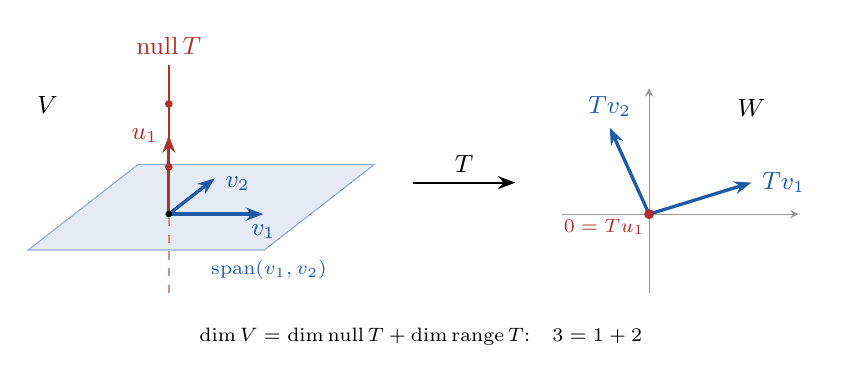
\begin{tikzpicture}[scale=1.0,>={Stealth[length=2.2mm]}]
\begin{scope}[x={(1cm,0cm)},y={(0.45cm,0.35cm)},z={(0cm,1cm)}]
\fill[figB!12] (-1.2,-1.3,0)--(1.8,-1.3,0)--(1.8,1.8,0)--(-1.2,1.8,0)--cycle;
\draw[figB!50] (-1.2,-1.3,0)--(1.8,-1.3,0)--(1.8,1.8,0)--(-1.2,1.8,0)--cycle;
\node[figB,font=\scriptsize,anchor=north west] at (1.0,-1.3,0) {$\operatorname{span}(v_1,v_2)$};
\draw[figR!55,thick,dashed] (0,0,-1.0)--(0,0,0);
\draw[figR,thick] (0,0,0)--(0,0,1.9) node[above,font=\small]{$\operatorname{null}T$};
\foreach \z in {0.6,1.4} \fill[figR] (0,0,\z) circle (1.4pt);
\draw[->,very thick,figR] (0,0,0)--(0,0,1) node[left,font=\small]{$u_1$};
\draw[->,very thick,figB] (0,0,0)--(1.2,0,0) node[below,font=\small]{$v_1$};
\draw[->,very thick,figB] (0,0,0)--(0,1.3,0) node[right,font=\small,yshift=-2pt]{$v_2$};
\fill (0,0,0) circle (1.2pt);
\node[font=\small] at (-1.0,-1.2,1.8) {$V$};
\end{scope}
\draw[->,thick] (3.1,0.4)--(4.4,0.4) node[midway,above,font=\small]{$T$};
\begin{scope}[xshift=6.1cm]
\draw[-stealth,thin,black!40] (-1.1,0)--(1.9,0);
\draw[-stealth,thin,black!40] (0,-1.0)--(0,1.6);
\draw[->,very thick,figB] (0,0)--(1.3,0.4) node[right,font=\small]{$Tv_1$};
\draw[->,very thick,figB] (0,0)--(-0.5,1.1) node[above,font=\small]{$Tv_2$};
\fill[figR] (0,0) circle (1.8pt) node[below left,font=\scriptsize,figR,inner sep=1.5pt]{$0=Tu_1$};
\node[font=\small] at (1.3,1.35) {$W$};
\end{scope}
\node[font=\scriptsize,align=center] at (3.2,-1.55) {$\dim V=\dim\operatorname{null}T+\dim\operatorname{range}T$:\quad $3=1+2$};
\end{tikzpicture}
\end{document}
